\documentclass[french]{beamer}

\usepackage[utf8]{inputenc}
\usepackage[T1]{fontenc}
\usepackage{lmodern}
\usepackage{amsmath, amssymb}

\usepackage{babel}
\usepackage{listings}

%CHOIX DU THEME et/ou DE SA COULEUR
%\usetheme{PaloAlto}
%\usetheme{Madrid}

\usetheme{Copenhagen}
% => il est possible, pour un thème donné, de modifier seulement la couleur
%\usecolortheme{crane}
\usecolortheme{seahorse}
%\useoutertheme[left]{sidebar}

\title{Projet collaboratif : Pollen}
\subtitle{Partie Élasticité linéaire dans un domaine axisymétrique}
\author{Nabil Belahrach \& Alexandre Corizzi}
\date{Novembre 2015}
\institute{Université de Strasbourg -- U.F.R. de Mathèmatiques
et d'Informatique}

\begin{document}
\newcommand*\diff{\mathop{\!\mathrm{d}}}
\AtBeginSection[{\begin{frame}{Outline}
    \tableofcontents[hideothersubsections, pausesections] 
\end{frame}}]

\defverbatim[colored]
\lstI{
  \begin{lstlisting}[language=C++,basicstyle=\ttfamily,keywordstyle=\color{red}]
  fespace Vh( Th, [P2,P2] );
  Vh [ur,uz], [vr,vz];
  real sigma = 0; // value of the shift 

  varf a( [u1h,u2h], [v1h,v2h] )= 
  int2d(Th)( ... -sigma(u1h*v1h + u2h*v2h) )
  +on(2,4,u1h=0,u2h=0);

  varf b( [u1h,u2h], [v1h,v2h] )=
  int2d(Th)( u1h*v1h + u2h*v2h ) ;
  \end{lstlisting}
}

\defverbatim[colored]
\lstII{
  \begin{lstlisting}[language=C++,basicstyle=\ttfamily,keywordstyle=\color{red}]

  matrix A = a(Vh,Vh,solver=Crout,factorize=1); 
  matrix B = b(Vh,Vh,solver=CG,eps=1e-20); 

  int nev = 100;  
  real[int] ev(nev); 
  Vh[int] [vp1, vp2](nev); 

  int k = EigenValue(A,B,sym=true,sigma=sigma,
  value=ev,vector=vp1,tol=1e-10,maxit=0,ncv=0);

   \end{lstlisting}
}

\defverbatim[colored]
\lstIII{
  \begin{lstlisting}[language=C++,basicstyle=\ttfamily,keywordstyle=\color{red}]
  k = min(k, nev); 
  k.sort;
  for (int i=0;i<k;i++){
    [ur,uz]=[vp1[i], vp2[i]];
    cout << `` ---- '' <<  i<< `` '' 
    << ev[i] << endl ;
    plot([ur,uz],cmm=``Eigen  Vector ''+i
    +`` valeur ='' + ev[i],value=1,wait=1,dim=2);
  }
   \end{lstlisting}
}

\addtobeamertemplate{footline}{\insertframenumber/\inserttotalframenumber}

\begin{frame}
  \titlepage
\end{frame}
\begin{frame}{Plan}
  \tableofcontents
\end{frame}

% ------------------------------------------------------------------------------
\section{Présentation du problème}
\begin{frame}
  \vfill
  \centering
  \begin{beamercolorbox}[sep=8pt,center,shadow=true,rounded=true]{title}
    \usebeamerfont{title}\insertsectionhead
  \end{beamercolorbox}
  \vfill
\end{frame}
% ------------------------------------------------------------------------------

\begin{frame}{Schéma de la buse}
  \begin{center}
    \begin{figure}
      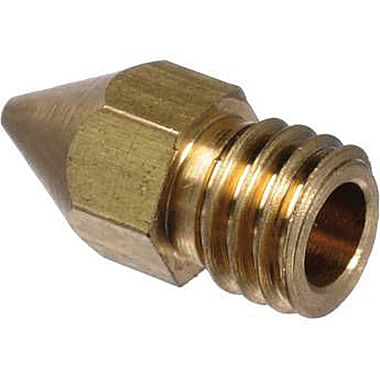
\includegraphics[scale=0.3]{images/buse.png}
      \caption{Buse reliée à la vis d'extrusion}
    \end{figure}
  \end{center}
\end{frame}

\begin{frame}{Schéma de la buse}
  \begin{minipage}{0.48\textwidth}
    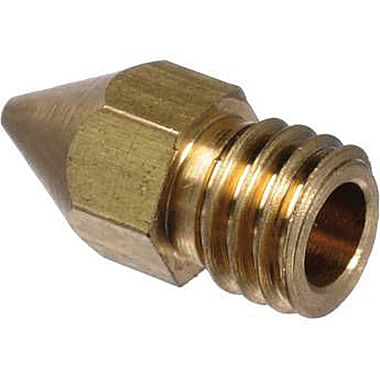
\includegraphics[scale=0.3]{images/buse.png}
  \end{minipage}
  \hspace*{\stretch{1}}
  \begin{minipage}{0.48\textwidth}
    Propriétés élastiques :
    \begin{itemize}
      \item Matériau homogéne isotrope
	\pause
      \item Loi de Hooke en 3D  
    \end{itemize}
  \end{minipage}
\end{frame}


\begin{frame}{Schéma de la buse}
  \begin{minipage}{0.48\textwidth}
    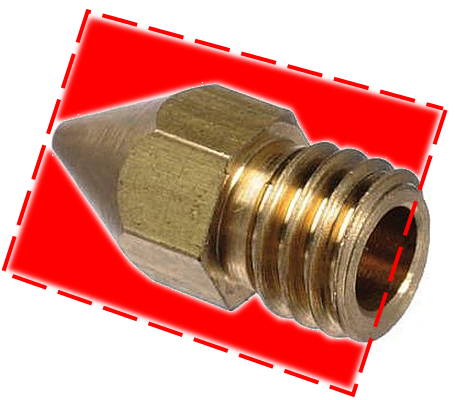
\includegraphics[scale=0.3]{images/buseCoupe.png}
  \end{minipage}
  \hspace*{\stretch{1}}
  \begin{minipage}{0.48\textwidth}
    Propriétés géométriques :
    \begin{itemize}
      \item Axisymétrique
	\pause
      \item Utilisation de Coordonnées cylindriques
	\pause
      \item Passage à un Problème 2D
    \end{itemize}
  \end{minipage}
\end{frame}

% ------------------------------------------------------------------------------

\section{Formulation des équations}
\begin{frame}
  \vfill
  \centering
  \begin{beamercolorbox}[sep=8pt,center,shadow=true,rounded=true]{title}
    \usebeamerfont{title}\insertsectionhead
  \end{beamercolorbox}
  \vfill
\end{frame}
% ------------------------------------------------------------------------------

\subsection{Principaux acteurs}
\begin{frame}{Déplacement et déformation}
  \begin{itemize}
    \item Vecteur de déplacement : $\vec{u}=(u_1,u_2,u_3) \in \mathbb{R}^3 $
  \end{itemize}
  \pause
  \vspace{2pt}

  \begin{equation}
    \nabla u =  
    \left(
    \begin{array}{ccc}
      \frac{\partial u_1}{\partial x } & \frac{\partial u_1}{\partial y } & 
      \frac{\partial u_1}{\partial z }  \\
      \frac{\partial u_2}{\partial x } & \frac{\partial u_2}{\partial y } & 
      \frac{\partial u_2}{\partial z }  \\
      \frac{\partial u_3}{\partial x } & \frac{\partial u_3}{\partial y } & 
      \frac{\partial u_3}{\partial z } 
    \end{array}
    \right)
  \end{equation}
  \pause
  \vspace{2pt}
  \begin{itemize}
    \item On définit le \emph{tenseur des déformations} symétrique : 
  \end{itemize}

  \begin{equation}
    \boxed{\varepsilon = \frac{1}{2} \left( \nabla u + ^{t} \nabla u \right)} 
    \in \mathcal{M}_{3,3}(\mathbb{R})
  \end{equation}

\end{frame}


\begin{frame}{Loi de Hooke}

   \emph{Relation linéaire entre une force et une déformation.}
   \pause
  \begin{equation}
    \sigma \left(\vec{u}\right) = \left( \lambda \hspace{2pt}\mathbf{div} 
    \hspace{2pt}\vec{u} \cdot \mathbf{I} \right) + 2 \mu\cdot \varepsilon 
  \end{equation}
  \begin{itemize}
      \pause
    \item $\lambda$ et $\mu$ sont les coefficients de Lamé du matériau. \\
      \pause
      $\mu$ est la résistance au cisaillement 
      \pause
     \item $\sigma \in \mathcal{M}_{3,3}(\mathbb{R})$ : tenseur des contraintes (efforts intérieurs)
    
  \end{itemize}
\end{frame}


\subsection{Problème aux Valeurs Propres} 
\begin{frame}{Problème aux Valeurs Propres} 
  \begin{itemize}
     \item Élasticité aux valeurs propres:
  \end{itemize}

  
%  \begin{equation*}
%    - \mathbf{div}  \left( \sigma \left(\vec{u}\right) \right) = \vec{\mathbf{F}}_{ext}
%  \end{equation*}

  \begin{equation}
   - \mathbf{div}  \left( \sigma \left(\vec{u}\right) \right) = \lambda_u \cdot \vec{u}
  \end{equation}
  \pause
    \begin{itemize}
     \item Avec les conditions aux bords suivantes:
  \end{itemize}

\[u_i = u_{0i} \quad \text{sur} \quad \Gamma_1 \text{,} \]
\pause
\[\sum_{j=1}^3 \sigma_{ij} n_j  = g_i \quad \text{sur} \quad \Gamma_2 \text{.}\]
  
\end{frame}

\subsection{Formulation faible}
\begin{frame}
  \begin{equation}
    - \int_\Omega \mathbf{div}  \left( \sigma \left(u\right) \right) v \hspace{7pt} \diff \Omega 
    = \lambda_u\int_\Omega  \hspace{2pt} u v \hspace{7pt} \diff \Omega
  \end{equation}
  \pause
  On a d'abord :
  \begin{equation*}
    \left[\mathbf{div}  \left( \sigma \left(\vec{u}\right) \right)\right]_i = 
    \sum_{j=1}^3 \frac{\partial\sigma_{i,j}}{\partial x_j}, \hspace{28pt}  \boxed{1 \leq i \leq 3}
      \end{equation*}
  \pause
  \vspace{10pt}
  Et donc : 
  \begin{equation}
    ^{\mathrm{GREEN}}\Leftrightarrow
      \int_\Omega \sum_{j=1}^3 \sigma_{i,j} \frac{\partial v_i}{\partial x_j} \diff \Omega 
      \underbrace{- \int_{\Gamma_{2}} \sum_{j=1}^3 \left(\sigma_{i,j}, \vec{\mathbf{n}} \right) v_i \hspace{7pt} 
       \diff {\Gamma_{2}}}_{\mathrm{BC}}
    = \lambda_u \int_\Omega  \hspace{2pt} u_i v_i \hspace{7pt} \diff \Omega
  \end{equation}
 \end{frame}
%---------------------------------------------------------------------
\begin{frame}
 \begin{itemize}
 \item conformément à La condition limite sur $\Gamma_{2}$

$$\int_{\Omega}\sum_{j=1}^{3}\sigma_{ij}\frac{\partial v_{i}}{\partial x_{j}} - \int_{\Gamma_{2}}g_{j}v_{i}  = \lambda_u\int_{\Omega} u_{i}v_{i},\hspace{0.2cm} pour : 1\leq i \leq 3$$ 
     \end{itemize}

\end{frame}
%-----------------------------------------------------------------------
\begin{frame}
    \begin{itemize}
    \item En détails : \\
    \end{itemize}
\begin{tiny}


 \begin{eqnarray}
\int_{\Omega} \left[\lambda \mbox{div}u + 2 \mu \frac{\partial u_1}{\partial x_1}\right] \frac{\partial v_1}{\partial x_1} + \mu \left(\frac{\partial u_1}{\partial x_2} + \frac{\partial u_2}{\partial x_1}\right)\frac{\partial v_1}{\partial x_2} + \mu \left(\frac{\partial u_1}{\partial x_3} + \frac{\partial u_3}{\partial x_1}\right)\frac{\partial v_1}{\partial x_3}
- \int_{\Gamma_2} g_1 v_1 = \lambda_u\int_{\Omega}u_1\ v_1,\nonumber\\
\int_{\Omega} \mu \left(\frac{\partial u_1}{\partial x_2} + \frac{\partial u_2}{\partial x_1}\right)\frac{\partial v_2}{\partial x_1} + \left[\lambda \mbox{div}u + 2 \mu \frac{\partial u_2}{\partial x_2}\right] \frac{\partial v_2}{\partial x_2} + \mu \left(\frac{\partial u_2}{\partial x_3} + \frac{\partial u_3}{\partial x_2}\right)\frac{\partial v_2}{\partial x_3}
- \int_{\Gamma_2} g_2 v_2 = \lambda_u\int_{\Omega}u_2\ v_2,\\
\int_{\Omega} \mu \left(\frac{\partial u_1}{\partial x_3} + \frac{\partial u_3}{\partial x_1}\right)\frac{\partial v_3}{\partial x_1} + \mu \left(\frac{\partial u_2}{\partial x_3} + \frac{\partial u_3}{\partial x_2}\right)\frac{\partial v_3}{\partial x_2}  + \left[\lambda \mbox{div}u + 2 \mu \frac{\partial u_3}{\partial x_3}\right] \frac{\partial v_3}{\partial x_3}
- \int_{\Gamma_2} g_3 v_3 = \lambda_u\int_{\Omega}u_3\ v_3.\nonumber
  \end{eqnarray}    
\end{tiny}


\end{frame}
%------------------------------------------------------------------------
\subsection{Changement de variables} 
\begin{frame}{Coordonnées cylindriques}
  \begin{minipage}{0.48\textwidth}
  
   \begin{itemize}
       \item Coordonnées cylindriques: \\
    \end{itemize}
$$g(x_1, x_2, x_3) = g(x_1(r, \phi), x_2(r, \phi), x_3(z))$$  

      \begin{equation}
	\left \{
	  \begin{array}{ccc}
	    x_1(r, \phi) &=& r \cos \phi  \\
	    x_2(r, \phi) & = & r \cos \phi   \\
	    x_3(z) & = & z \\
	  \end{array}
	  \right.
	\end{equation}
	
%    \begin{equation*}
%      \left \{
%	\begin{array}{ccc}
%	  x & = &r \cos \theta  \\
%	  y & = &r \sin \theta   \\
%	  z & = &z \\
%	\end{array}
%	\right.
%      \end{equation*}
    \end{minipage}
    \hspace*{\stretch{1}}
    \begin{minipage}{0.48\textwidth}
   
      \end{minipage}
      \pause
    \vspace{23pt}

\end{frame}

\begin{frame}

\begin{itemize}
  \item Les dérivées:
\end{itemize}

      \begin{equation}
	\left \{
	  \begin{array}{ccc}
\frac{\partial g}{\partial r} &=& \frac{\partial g}{\partial x_1}\cos\phi +  \frac{\partial g}{\partial x_2}\sin\phi \\
\frac{\partial g}{\partial \phi} &=& \frac{\partial g}{\partial x_1}(-r\sin\phi) +  \frac{\partial g}{\partial x_2}r\cos\phi\\
\frac{\partial g}{\partial z} &=& \frac{\partial g}{\partial x_3}
	  \end{array}
	  \right.
	\end{equation}
	
\pause 
\begin{itemize}
  \item De là, nous obtenons
\end{itemize}

	
      \begin{equation}
	\left \{
	  \begin{array}{ccc}

\frac{\partial g}{\partial x_1} &=& \frac{\partial g}{\partial r}\cos\phi - \frac{1}{r}\frac{\partial g}{\partial \phi}\sin\phi,\nonumber \\
\frac{\partial g}{\partial x_2} &=& \frac{\partial g}{\partial r}\sin\phi + \frac{1}{r}\frac{\partial g}{\partial \phi}\cos\phi, \\
\frac{\partial g}{\partial x_3} &=& \frac{\partial g}{\partial z}. \nonumber
	  \end{array}
	  \right.
	\end{equation}
\end{frame}	


% ------------------------------------------------------------------------------

\begin{frame} 

\begin{itemize}
  \item De manière analogue:


	
      \begin{equation*}
	\left \{
	  \begin{array}{ccc}
\frac{\partial u_1}{\partial x_1} &=& \frac{\partial u_r}{\partial r}\cos^2\phi + \frac{1}{r} u_r\sin^2\phi,\nonumber \\
\frac{\partial u_1}{\partial x_2} &=& \frac{\partial u_r}{\partial r}\cos\phi\sin\phi - \frac{1}{r}u_r \cos\phi\sin\phi, \nonumber \\
\frac{\partial u_1}{\partial x_3} &=&\frac{\partial u_r}{\partial z}\cos\phi. \nonumber
	  \end{array}
	  \right.
	\end{equation*}
	
\pause
 \item De même pour $u_2$:
      \begin{equation*}
	\left \{
	  \begin{array}{ccc}

\frac{\partial u_2}{\partial x_1} &=& \frac{\partial u_r}{\partial r}\cos\phi\sin\phi - \frac{1}{r}u_r \cos\phi\sin\phi \\
\frac{\partial u_2}{\partial x_2} &=& \frac{\partial u_r}{\partial r}\sin^2\phi + \frac{1}{r} u_r\cos^2\phi \\
\frac{\partial u_2}{\partial x_3} &=& \frac{\partial u_r}{\partial z}\sin\phi
	  \end{array}
	  \right.
	\end{equation*}

	
  \end{itemize}
\end{frame}	

%--------------------------------------------------------------------------------

\begin{frame}
  \begin{itemize}
 \item Et finalement $u_3$
 
       \begin{equation*}
	\left \{
	  \begin{array}{ccc}	  
\frac{\partial u_3}{\partial x_1} &=& \frac{\partial u_z}{\partial r}\cos\phi, \nonumber \\
\frac{\partial u_3}{\partial x_2} &=& \frac{\partial u_z}{\partial r}\sin\phi,\nonumber \\
\frac{\partial u_3}{\partial x_3} &=& \frac{\partial u_z}{\partial z}. \nonumber
	  \end{array}
	  \right.
	\end{equation*}
  \end{itemize}
\end{frame}

%-------------------------------------------------------------------------------
\begin{frame}
 \begin{itemize}
 
   \item  Nous pouvons commencer à transformer les intégrales:
   
   \begin{tiny}
   
   
   \begin{eqnarray*} \int_{\Omega} r \left[\lambda (\frac{\partial u_r}{\partial r} + \frac{1}{r} u_r + \frac{\partial u_z}{\partial z}) + 2 \mu (\frac{\partial u_r}{\partial r}\cos^2\phi + \frac{1}{r} u_r\sin^2\phi)\right] (\frac{\partial v_r}{\partial r}\cos^2\phi + \frac{1}{r} v_r\sin^2\phi) + \\ r 2 \mu \left(\frac{\partial u_r}{\partial r}\cos\phi\sin\phi - \frac{1}{r}u_r \cos\phi\sin\phi\right)\left(\frac{\partial v_r}{\partial r}\cos\phi\sin\phi - \frac{1}{r}v_r \cos\phi\sin\phi\right) + \\ r \mu \left(\frac{\partial u_r}{\partial z}\cos\phi + \frac{\partial u_z}{\partial r}\cos\phi\right)\frac{\partial v_r}{\partial z}\cos\phi - \int_{\Gamma_2} r g_r v_r {\cos}^2 \phi = \lambda_u \int_{\Omega} r u_r\ v_r \cos^2 \phi, \end{eqnarray*}
   
   
   \end{tiny}
 \end{itemize}


\end{frame}


%-------------------------------------------------------------------------------
\begin{frame}

 \begin{itemize}
   \item La deuxième:
 \end{itemize}

\begin{tiny}
\begin{eqnarray*} 
\int_{\Omega} r 2\mu \left(\frac{\partial u_r}{\partial r}\cos\phi\sin\phi - \frac{1}{r}u_r \cos\phi\sin\phi\right)\left(\frac{\partial v_r}{\partial r}\cos\phi\sin\phi - \frac{1}{r}v_r \cos\phi\sin\phi\right) +\\  r \left[\lambda (\frac{\partial u_r}{\partial r} + \frac{1}{r} u_r + \frac{\partial u_z}{\partial z}) + 2 \mu (\frac{\partial u_r}{\partial r}\sin^2\phi + \frac{1}{r} u_r\cos^2\phi)\right] (\frac{\partial v_r}{\partial r}\sin^2\phi + \frac{1}{r} v_r\cos^2\phi) + \\  r \mu \left(\frac{\partial u_r}{\partial z}\sin\phi + \frac{\partial u_z}{\partial r}\sin\phi\right)(\frac{\partial v_r}{\partial z}\sin\phi)  - \int_{\Gamma_2}r g_r v_r \sin^2 \phi =\lambda_u \int_{\Omega}r u_r\ v_r \sin^2 \phi,\\ \end{eqnarray*} 
\end{tiny}

\end{frame}

%-------------------------------------------------------------------------------
\begin{frame}

 \begin{itemize}
   \item  On additionnes les deux formulations faibles.
   \item  Et pour simplifier $\phi = 0$. 
   \item $\Omega_0 = \Omega \cap $ \{\ le demi plan ${x_1}^{+} x_3$\}\ \\
  \end{itemize}
\pause
   \begin{tiny}
$$\int_{\Omega_0} r \lambda (\frac{\partial u_r}{\partial r} + \frac{1}{r} u_r + \frac{\partial u_z}{\partial z}) (\frac{\partial v_r}{\partial r} + \frac{1}{r} v_r) + \int_{\Omega_0} r \mu \left[ 2 \left(\frac{\partial u_r}{\partial r}\frac{\partial v_r}{\partial r} + \frac{1}{r^2} u_r v_r\right) +  \left(\frac{\partial u_r}{\partial z}\frac{\partial v_r}{\partial z} + \frac{\partial u_z}{\partial r}\frac{\partial v_r}{\partial z}\right)\right]$$ \\
$$ - \int_{\Gamma_2} g_r v_r r = \lambda_u \int_{\Omega_0} u_r\ v_r r $$ \\ 

   \end{tiny}
\end{frame}
%-----------------------------------------------------------------------------

\begin{frame}

 \begin{itemize}
   \item  Et enfin la formulation faible suivant $\vec {oz}$:
  \end{itemize}

   \begin{tiny}
$$\int_{\Omega_0} r \mu (\frac{\partial u_{r}}{\partial z}\frac{\partial v_{z}}{\partial r} + \frac{\partial u_{z}}{\partial r}\frac{\partial v_{z}}{\partial r} + 2 
\frac{\partial u_{z}}{\partial z}\frac{\partial v_{z}}{\partial z}) +
r\mu(\frac{\partial u_{r}}{\partial r}+ \frac{1}{r} u_{r} + \frac{\partial u_{z}}{\partial z}) \frac{\partial v_{z}}{\partial z}
-\int_{\Gamma_{2}} g_{z}v_{z}r  
= \lambda_u \int_{\Omega_0} u_{z}v_{z}r$$
   \end{tiny}

\end{frame}




% \begin{itemize}
% 
%   \item  Le deuxième intégrale: 
%   
%   \begin{tiny}
%   
%   
%\begin{eqnarray} \int_{\Omega} r 2\mu \left(\frac{\partial u_r}{\partial r}\cos\phi\sin\phi - \frac{1}{r}u_r \cos\phi\sin\phi\right)\left(\frac{\partial v_r}{\partial r}\cos\phi\sin\phi - \frac{1}{r}v_r \cos\phi\sin\phi\right) +\\  r \left[\lambda (\frac{\partial u_r}{\partial r} + \frac{1}{r} u_r + \frac{\partial u_z}{\partial z}) + 2 \mu (\frac{\partial u_r}{\partial r}\sin^2\phi + \frac{1}{r} u_r\cos^2\phi)\right] (\frac{\partial v_r}{\partial r}\sin^2\phi + \frac{1}{r} v_r\cos^2\phi) + \\  r \mu \left(\frac{\partial u_r}{\partial z}\sin\phi + \frac{\partial u_z}{\partial r}\sin\phi\right)(\frac{\partial v_r}{\partial z}\sin\phi)  - \int_{\Gamma_2}r g_r v_r \sin^2 \phi = \lambda_u \int_{\Omega}r u_r\ v_r \sin^2 \phi,\\ \end{eqnarray}
%     
%   \end{tiny}
% \end{itemize}
%
%
%\end{frame}
%%-------------------------------------------------------------------------------
  \section{Éxpérimentation}
  \begin{frame}
    \vfill
    \centering
    \begin{beamercolorbox}[sep=8pt,center,shadow=true,rounded=true]{title}
      \usebeamerfont{title}\insertsectionhead
    \end{beamercolorbox}
    \vfill
  \end{frame}
% ------------------------------------------------------------------------------
  \begin{frame}{Code FreeFem++}
	\lstI
  \end{frame}
% ------------------------------------------------------------------------------
  \begin{frame}{Code FreeFem++}
	\lstII
  \end{frame}
% ------------------------------------------------------------------------------
  \begin{frame}{Code FreeFem++}
	\lstIII
  \end{frame}

\begin{frame}
  \begin{center}
    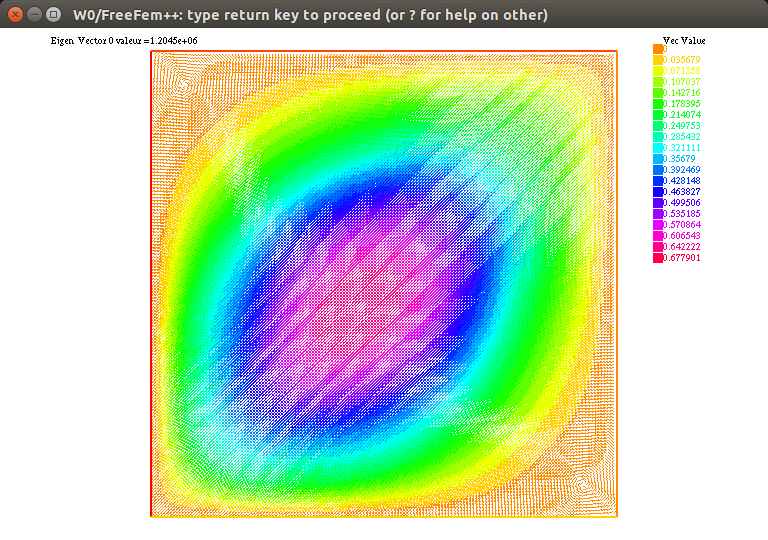
\includegraphics[scale=0.40]{images/WF_p1d.png}
  \end{center}
\end{frame}

\begin{frame}
  \begin{center}
    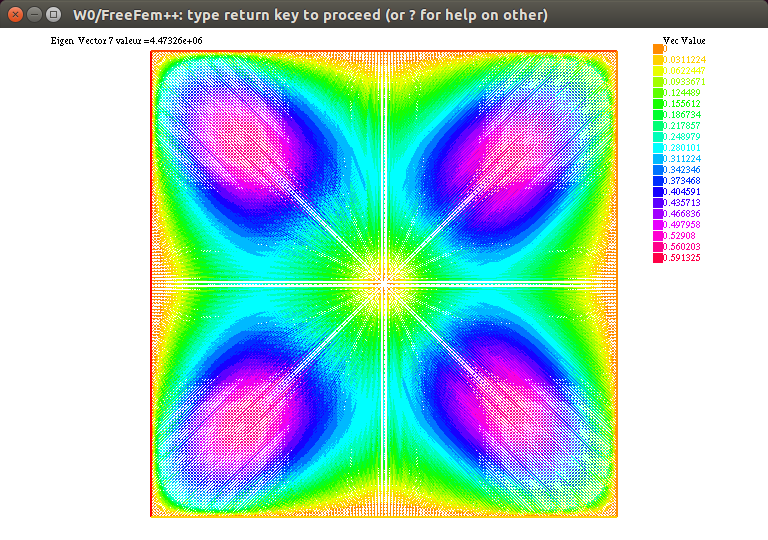
\includegraphics[scale=0.4]{images/WF_p2d.png}
  \end{center}
\end{frame}

\begin{frame}
  \begin{center}
    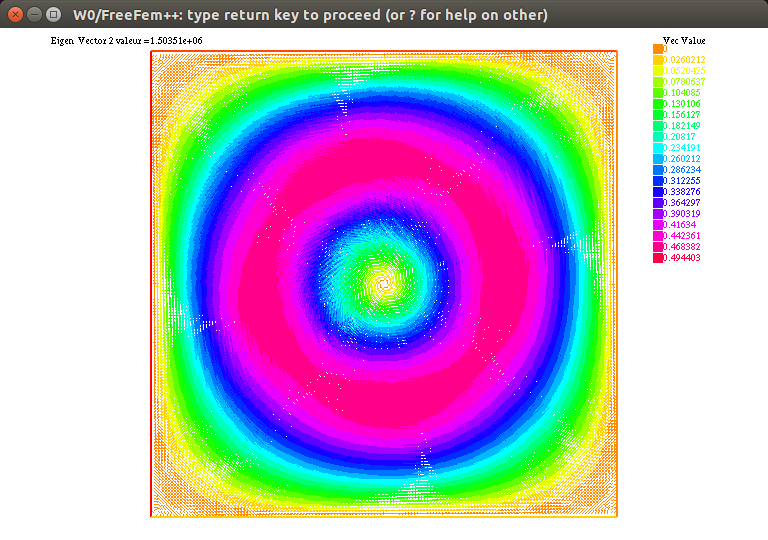
\includegraphics[scale=0.4]{images/WF_p3d.png}
  \end{center}
\end{frame}

\begin{frame}
  \begin{center}
    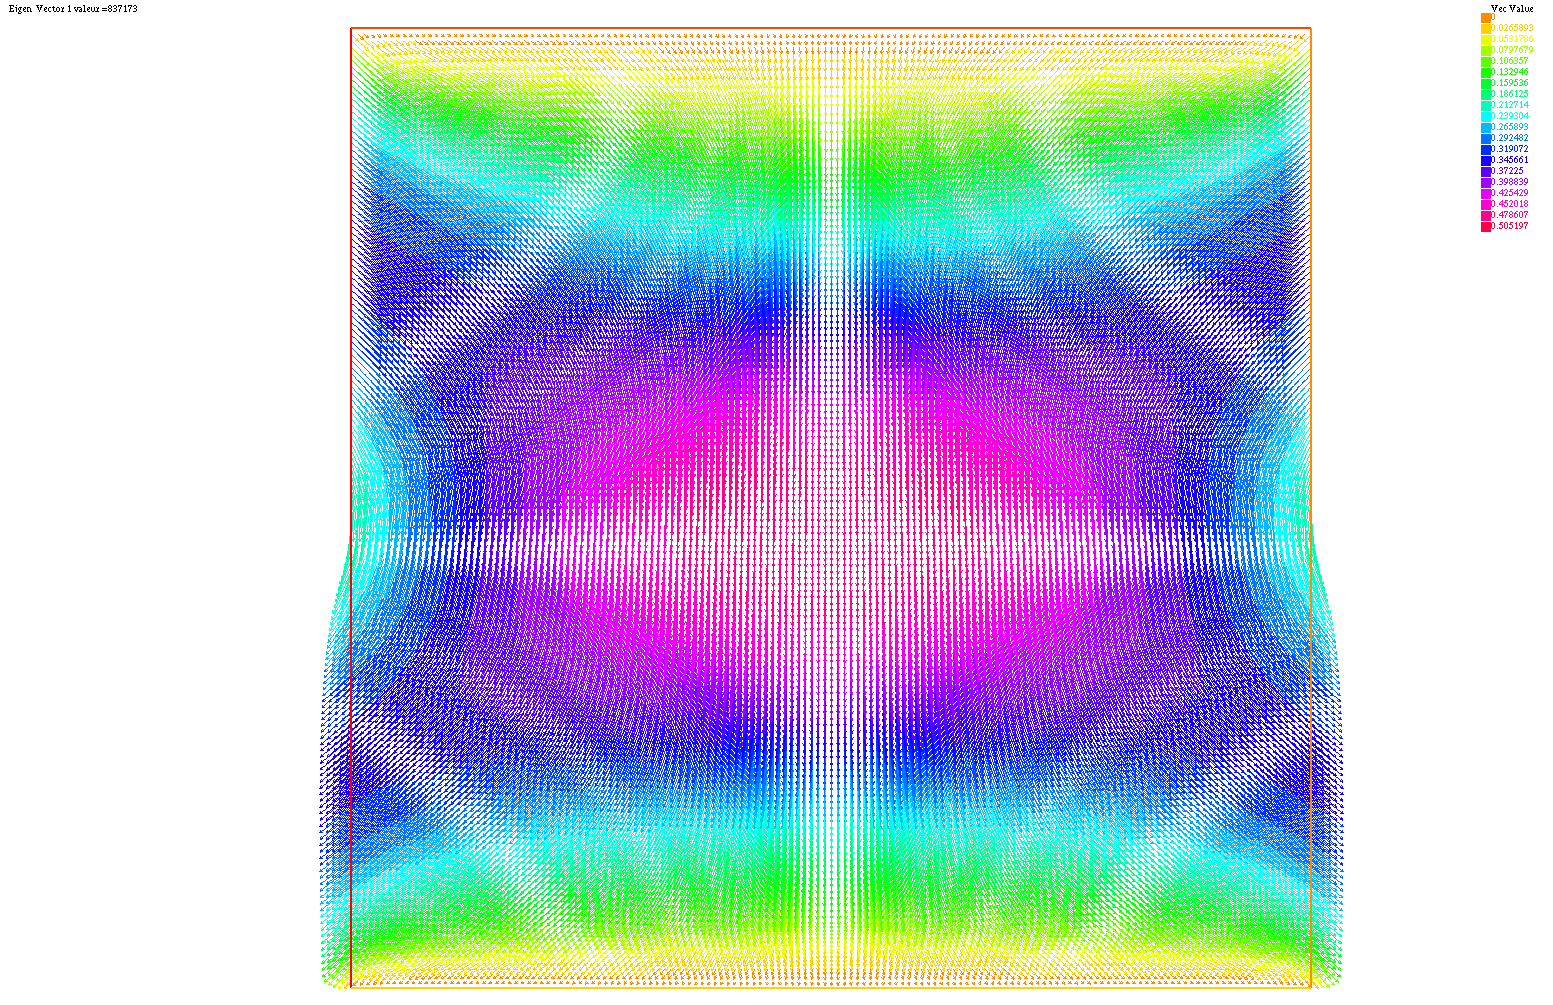
\includegraphics[scale=0.19]{images/WF_p1n.png}
  \end{center}
\end{frame}

\begin{frame}
  \begin{center}
    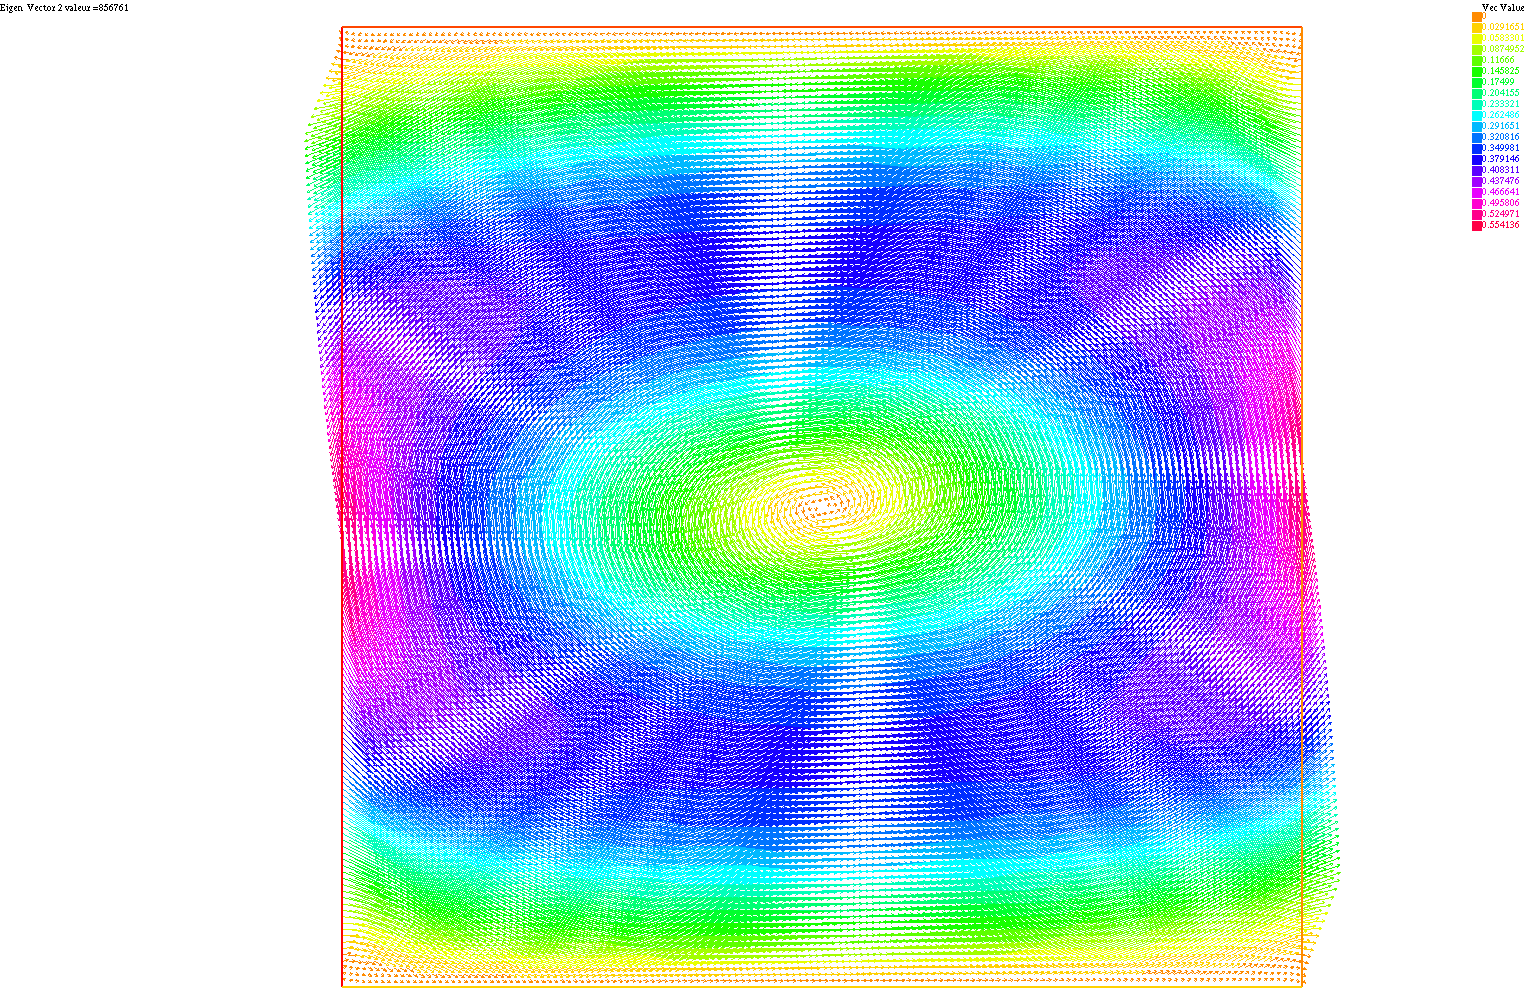
\includegraphics[scale=0.19]{images/WF_p2n.png}
  \end{center}
\end{frame}

\begin{frame}
  \begin{center}
    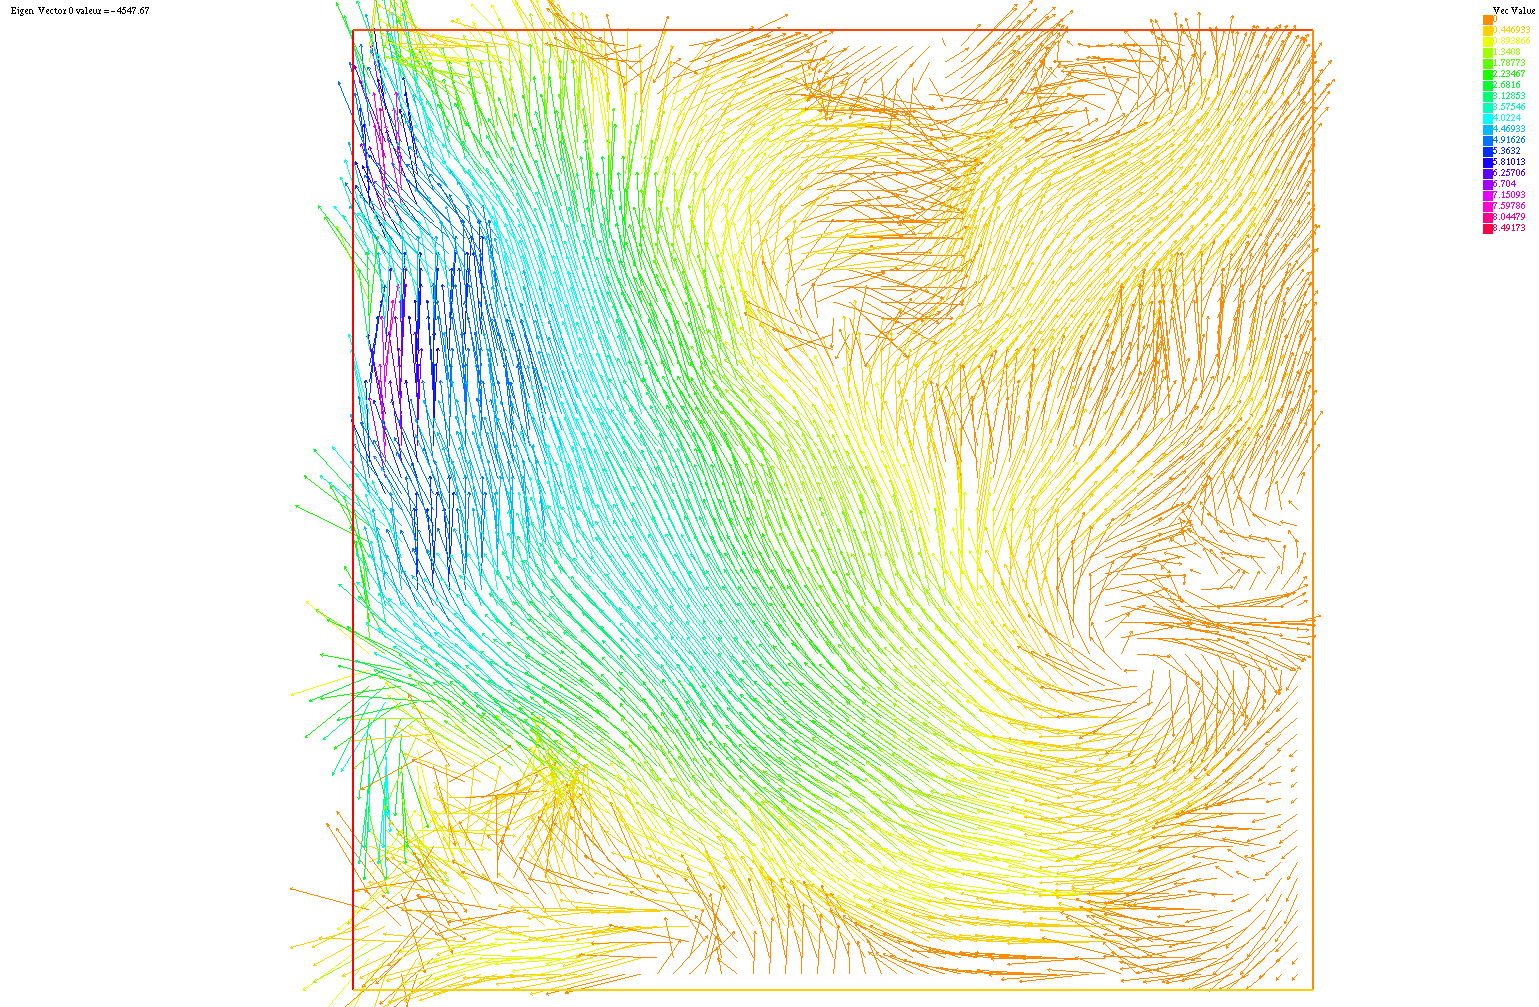
\includegraphics[scale=0.19]{images/WF.png}
  \end{center}
\end{frame}



\end{document}
